\documentclass{article}

% if you need to pass options to natbib, use, e.g.:
%     \PassOptionsToPackage{numbers, compress}{natbib}
% before loading neurips_2019

% ready for submission
% \usepackage{neurips_2019}

% to compile a preprint version, e.g., for submission to arXiv, add add the
% [preprint] option:
%     \usepackage[preprint]{neurips_2019}

% to compile a camera-ready version, add the [final] option, e.g.:
     \usepackage[final]{neurips_2019}

% to avoid loading the natbib package, add option nonatbib:
%     \usepackage[nonatbib]{neurips_2019}

\usepackage[utf8]{inputenc} % allow utf-8 input
\usepackage[T1]{fontenc}    % use 8-bit T1 fonts
\usepackage{hyperref}       % hyperlinks
\usepackage{url}            % simple URL typesetting
\usepackage{booktabs}       % professional-quality tables
\usepackage{amsfonts}       % blackboard math symbols
\usepackage{nicefrac}       % compact symbols for 1/2, etc.
\usepackage{microtype}      % microtypography
\usepackage{graphicx}
\usepackage{hyperref}
\hypersetup{
    colorlinks=true,
    linkcolor=blue,
    filecolor=magenta,      
    urlcolor=blue,
    citecolor=black
}
\usepackage{caption}
\usepackage{subcaption}

\title{Replicating Application of Elastic Weight Consolidation to Scrambled MNIST}

% The \author macro works with any number of authors. There are two commands
% used to separate the names and addresses of multiple authors: \And and \AND.
%
% Using \And between authors leaves it to LaTeX to determine where to break the
% lines. Using \AND forces a line break at that point. So, if LaTeX puts 3 of 4
% authors names on the first line, and the last on the second line, try using
% \AND instead of \And before the third author name.

\author{
	Oliver Spohngellert
}

\begin{document}

\maketitle

\begin{abstract}
	Catastrophic forgetting refers to the tendency of Neural Networks to "forget" previously learned information when they are trained on new information. In "Overcoming catastrophic forgetting in neural networks", the authors propose Elastic Weight Consolidation as a method for mitigating catastrophic forgetting. In this work, we attempt to replicate the results of the MNIST experiments in the aforementioned paper, specifically plots 2 A-C. We succeed in replicating plots 2A and 2C, but are not able to completely replicate the results of plot 2B.
\end{abstract}

\section{Introduction}

Catastrophic forgetting is a common problem for Deep Learning practitioners. Catastrophic forgetting occurs when a neural network is trained on multiple tasks sequentially, and the network "forgets" how to perform earlier tasks, resulting in poorer performance. This problem has been mentioned as early as 1989 in "Catastrophic Interference in Connectionist Networks: The Sequential Learning Problem" \cite{cfo1989}. One proposed solution to this problem is the use of pretraining. In "Catastrophic Interference is Eliminated in Pretrained Networks", the authors demonstrate that using a pretrained network helps reduce error on sequential tasks \cite{pretrain}. More recently, it has been shown that the use of Generative Replay can alleviate the problem, but it has the drawback of linearly increasing training time with the number of former tasks \cite{generative}.

In "Overcoming catastrophic forgetting in neural networks", the authors attempt to solve this problem by introducing Elastic Weight Consolidation (EWC) \cite{ewc}. EWC works by adding a regularization term that penalizes the network for straying too far from important weights in the network. This is done as follows:

$$
L(\theta) = L_{B}(\theta) + \frac{\lambda}{2} \sum_{i}F_{i}(\theta_{i} - \theta^{*}_{A,i})^2
$$

Where $L_{B}$ refers to the loss for task $B$ (the current task), $F_i$ refers to the diagonal of the fisher information matrix for weight $i$, and $\theta^{*}_{A,i}$ refers to the $i$th weight of the previous task $A$. This solution to catastrophic forgetting comes with the benefit of not requiring major changes to training procedure, robustness, and being fairly easy to implement. 

In order to prove the efficacy of EWC, the authors conducted experiments when using EWC on the MNIST dataset. In these experiments, they trained neural networks on the MNIST dataset, where the pixels in the images have been scrambled, and they produced the following figure:

\begin{figure}[h]
\centering
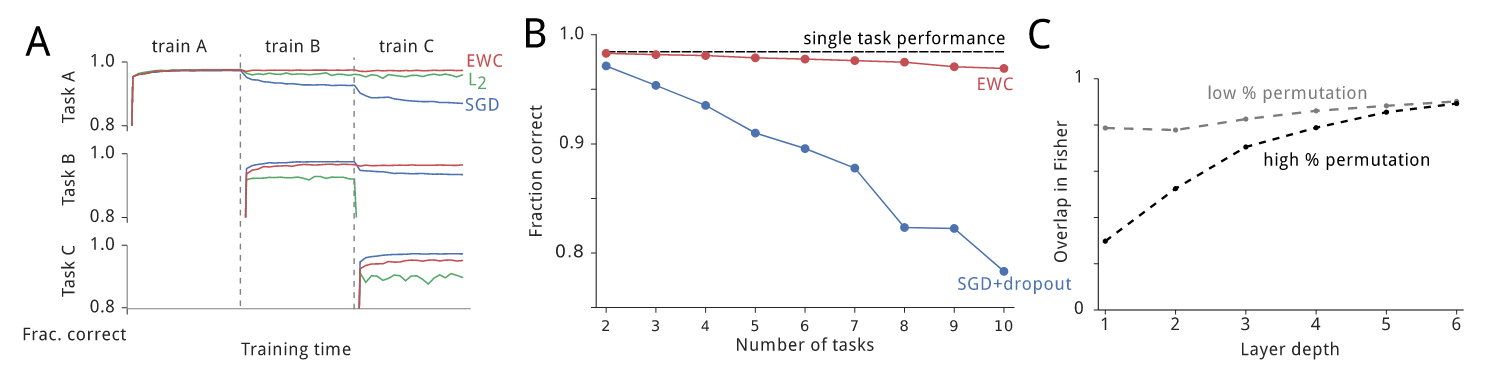
\includegraphics[scale=0.25]{../Figures/Orig_All.png}
\caption{The figure produced in the original paper}
\label{fig:orig_all}
\end{figure}

The main goal of this work was to reproduce the above figure.

\section{Implementation}

In order to replicate the figure in the original paper, EWC, L2 regularization by previous weights, random scrambling, calculation of the fisher diagonal, and training code had to be implemented. The full code can be found \href{http://www.overleaf.com}{here}. Below I will describe the general implementation approach.


\subsection{EWC and L2}

The fisher diagonal was calculated using the empirical fisher method, whose formula can be found in "Limitations of the Empirical Fisher Approximation for Natural Gradient Descent" \cite{empirical}. Once the fisher diagonal was calculated on the training set, this was passed to a class called "EWC", along with a replica of the model after training on the task. These together were used to calculate the regularization term in EWC using PyTorch operations in order to allow for differentiation. L2 had a similar implementation but only used the previous nets and no fisher matrix. The only difference I had from the original paper was using the norm of the regularization sum (adding a square root term), as I found this allowed for a greater range of lambda values to be used. The implementation of these classes, along with the scrambling code can be found \href{http://example.com}{here}.

\subsection{Training Code}

For each plot I implemented separate training loops, as different information needed to be saved for each, and they each used different network architectures. The majority of the hyperparameters used in the original paper were detailed, which allowed for a relatively painless implementation. However, the batch size and $\lambda$ hyperparameters were not listed. For batch size, I assumed a batch size of 1, and used this when possible, but for plots B and C batch size was increased to save computation time. $\lambda$ was set to 0.01 for plots A and C, and 0.01 or 0.005 for plot B. Further, the hyperparameters for plot B included a range of values, and the authors said they used a search for the optimal values. To save time, I used the middle value (1200) for hidden layer size, and the max value ($10^{-3}$) for learning rate. The implementations of training loops for each plot can be found at the following locations: \href{}{Plot A}, \href{}{Plot B}, \href{}{Plot C}. 

\subsection{Plotting}

Once the data was saved, re-loaded and plotted. For plot C, the metric for overlap in fisher was "Fr\' echet Distance". The formula for this can be found in section 4.3 of the original paper, and this formula was used. The implementation of these plots can be found \href{}{here}.

\section{Results}

\begin{figure}[!h]
     \centering
     \begin{subfigure}[b]{0.32\textwidth}
         \centering
         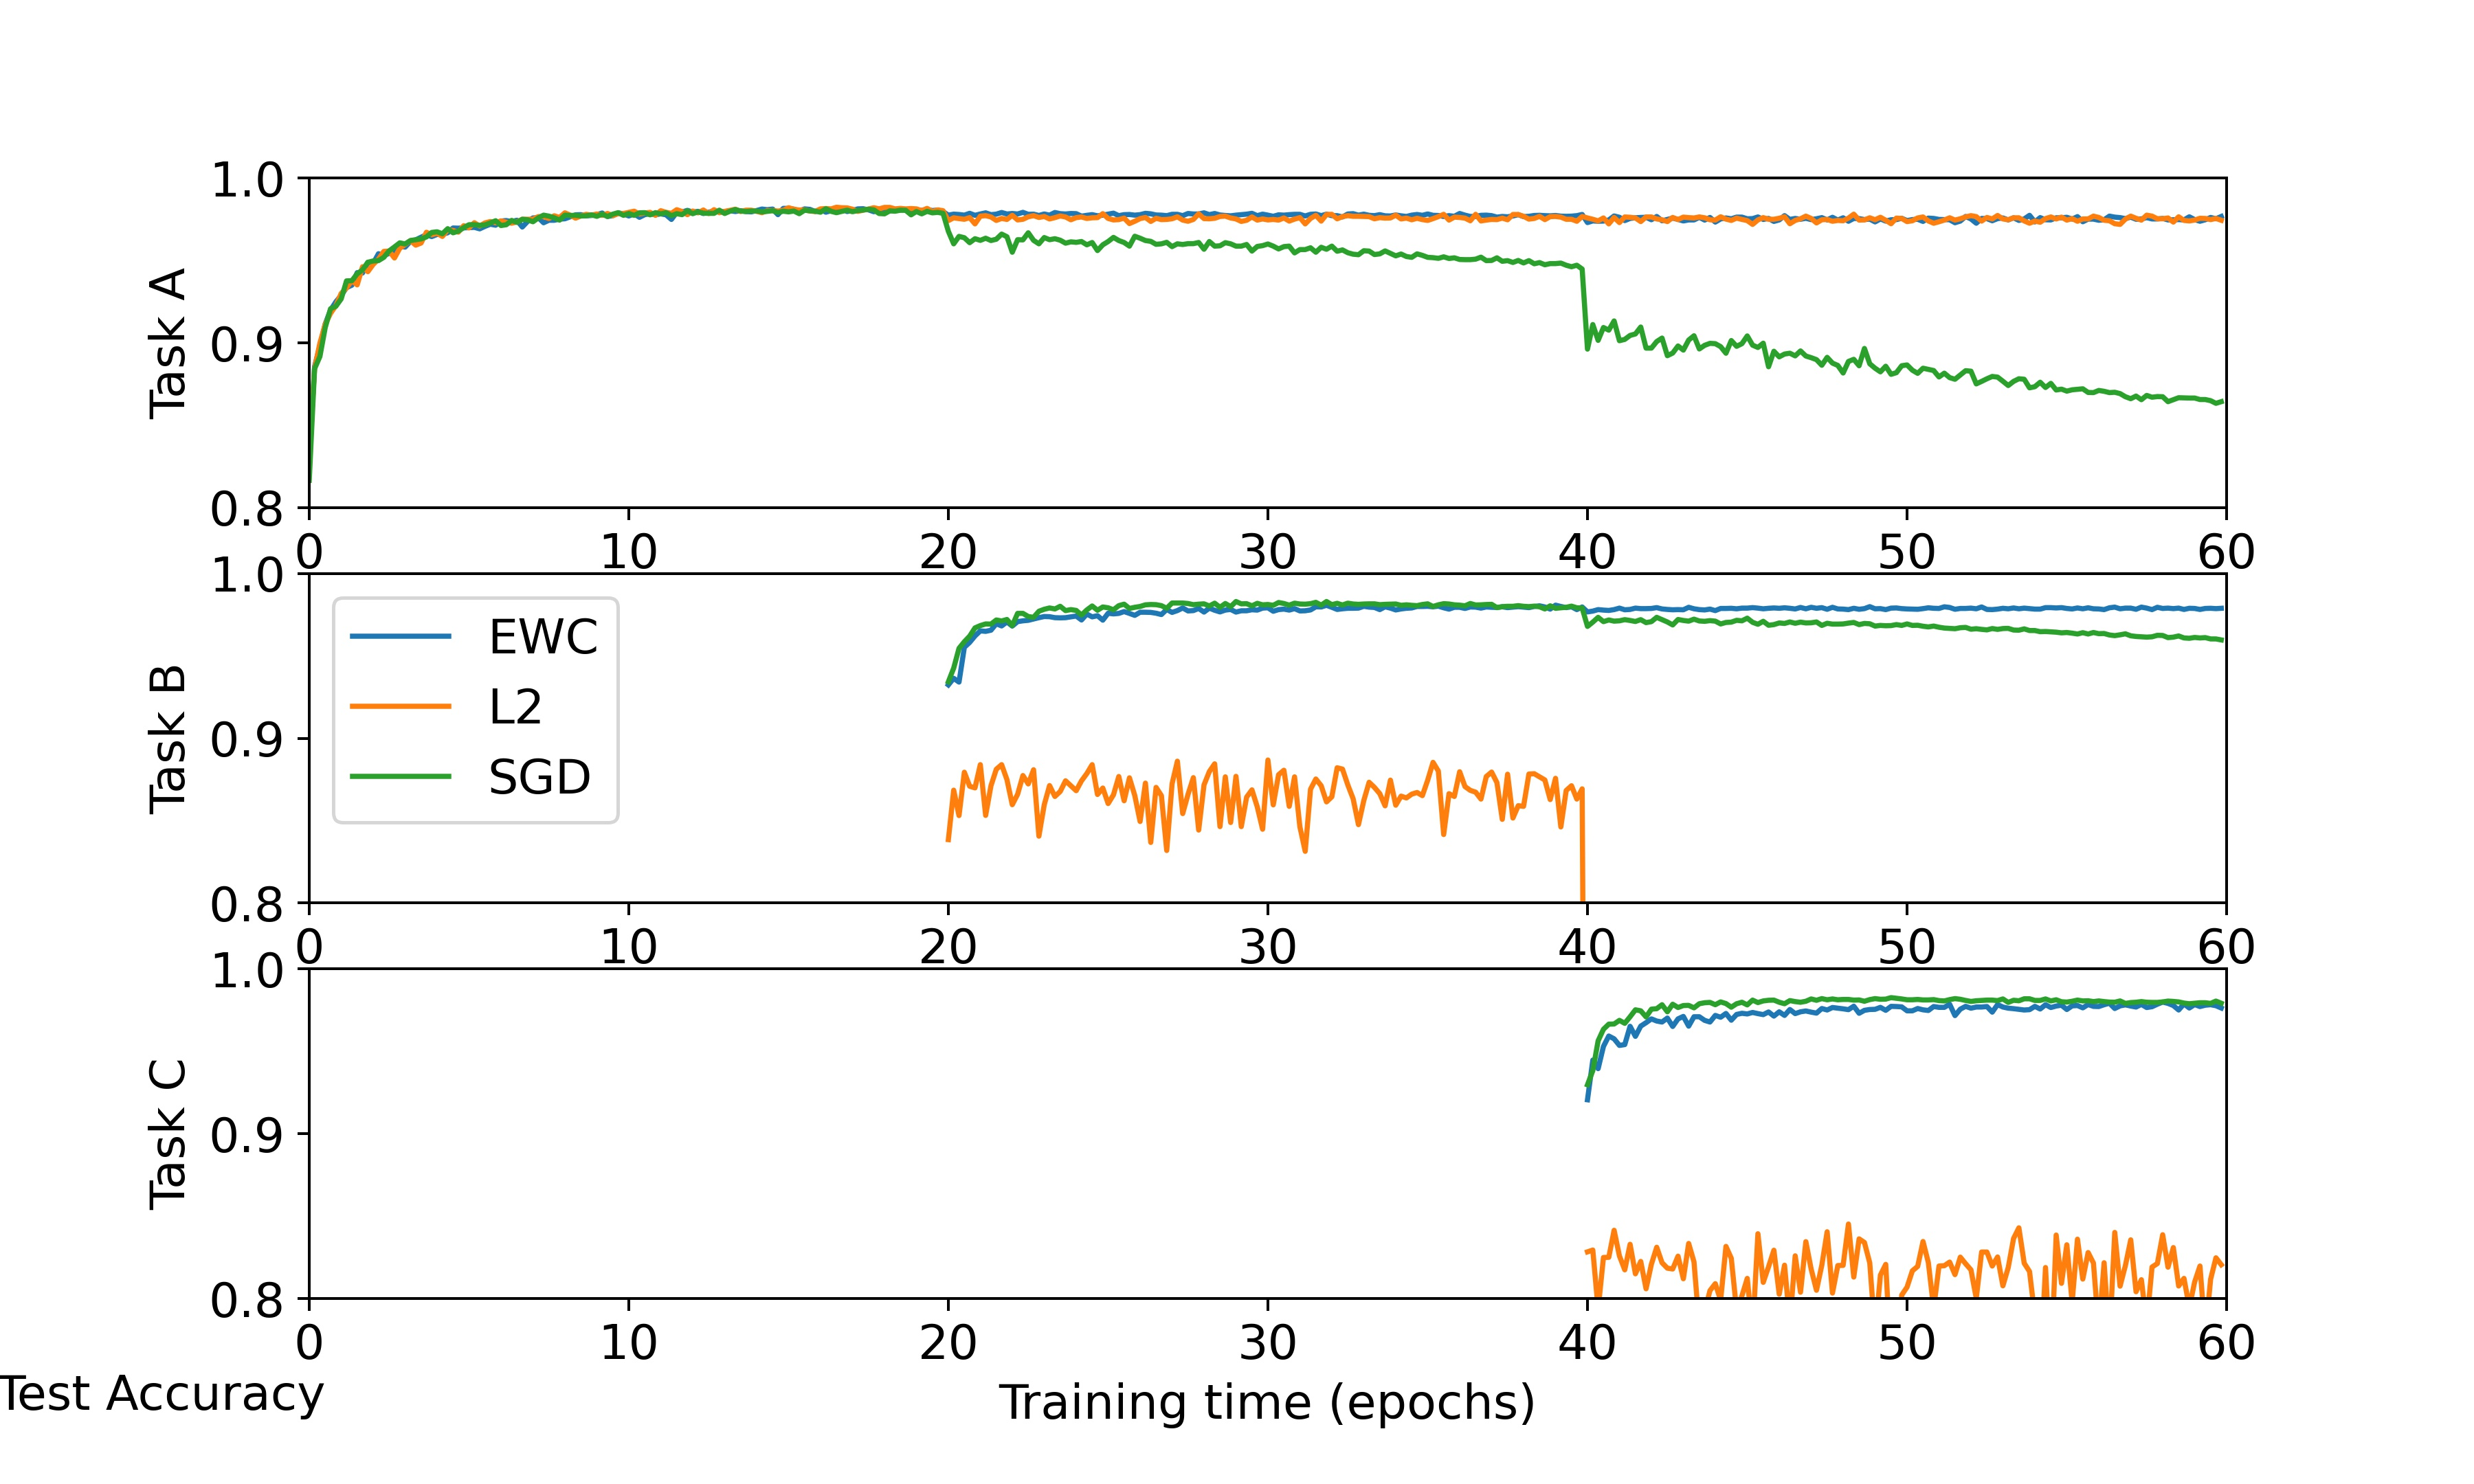
\includegraphics[width=\textwidth]{../Figures/Plot_a.jpg}
         \caption{}
         \label{fig:repa}
     \end{subfigure}
     \hfill
     \begin{subfigure}[b]{0.32\textwidth}
         \centering
         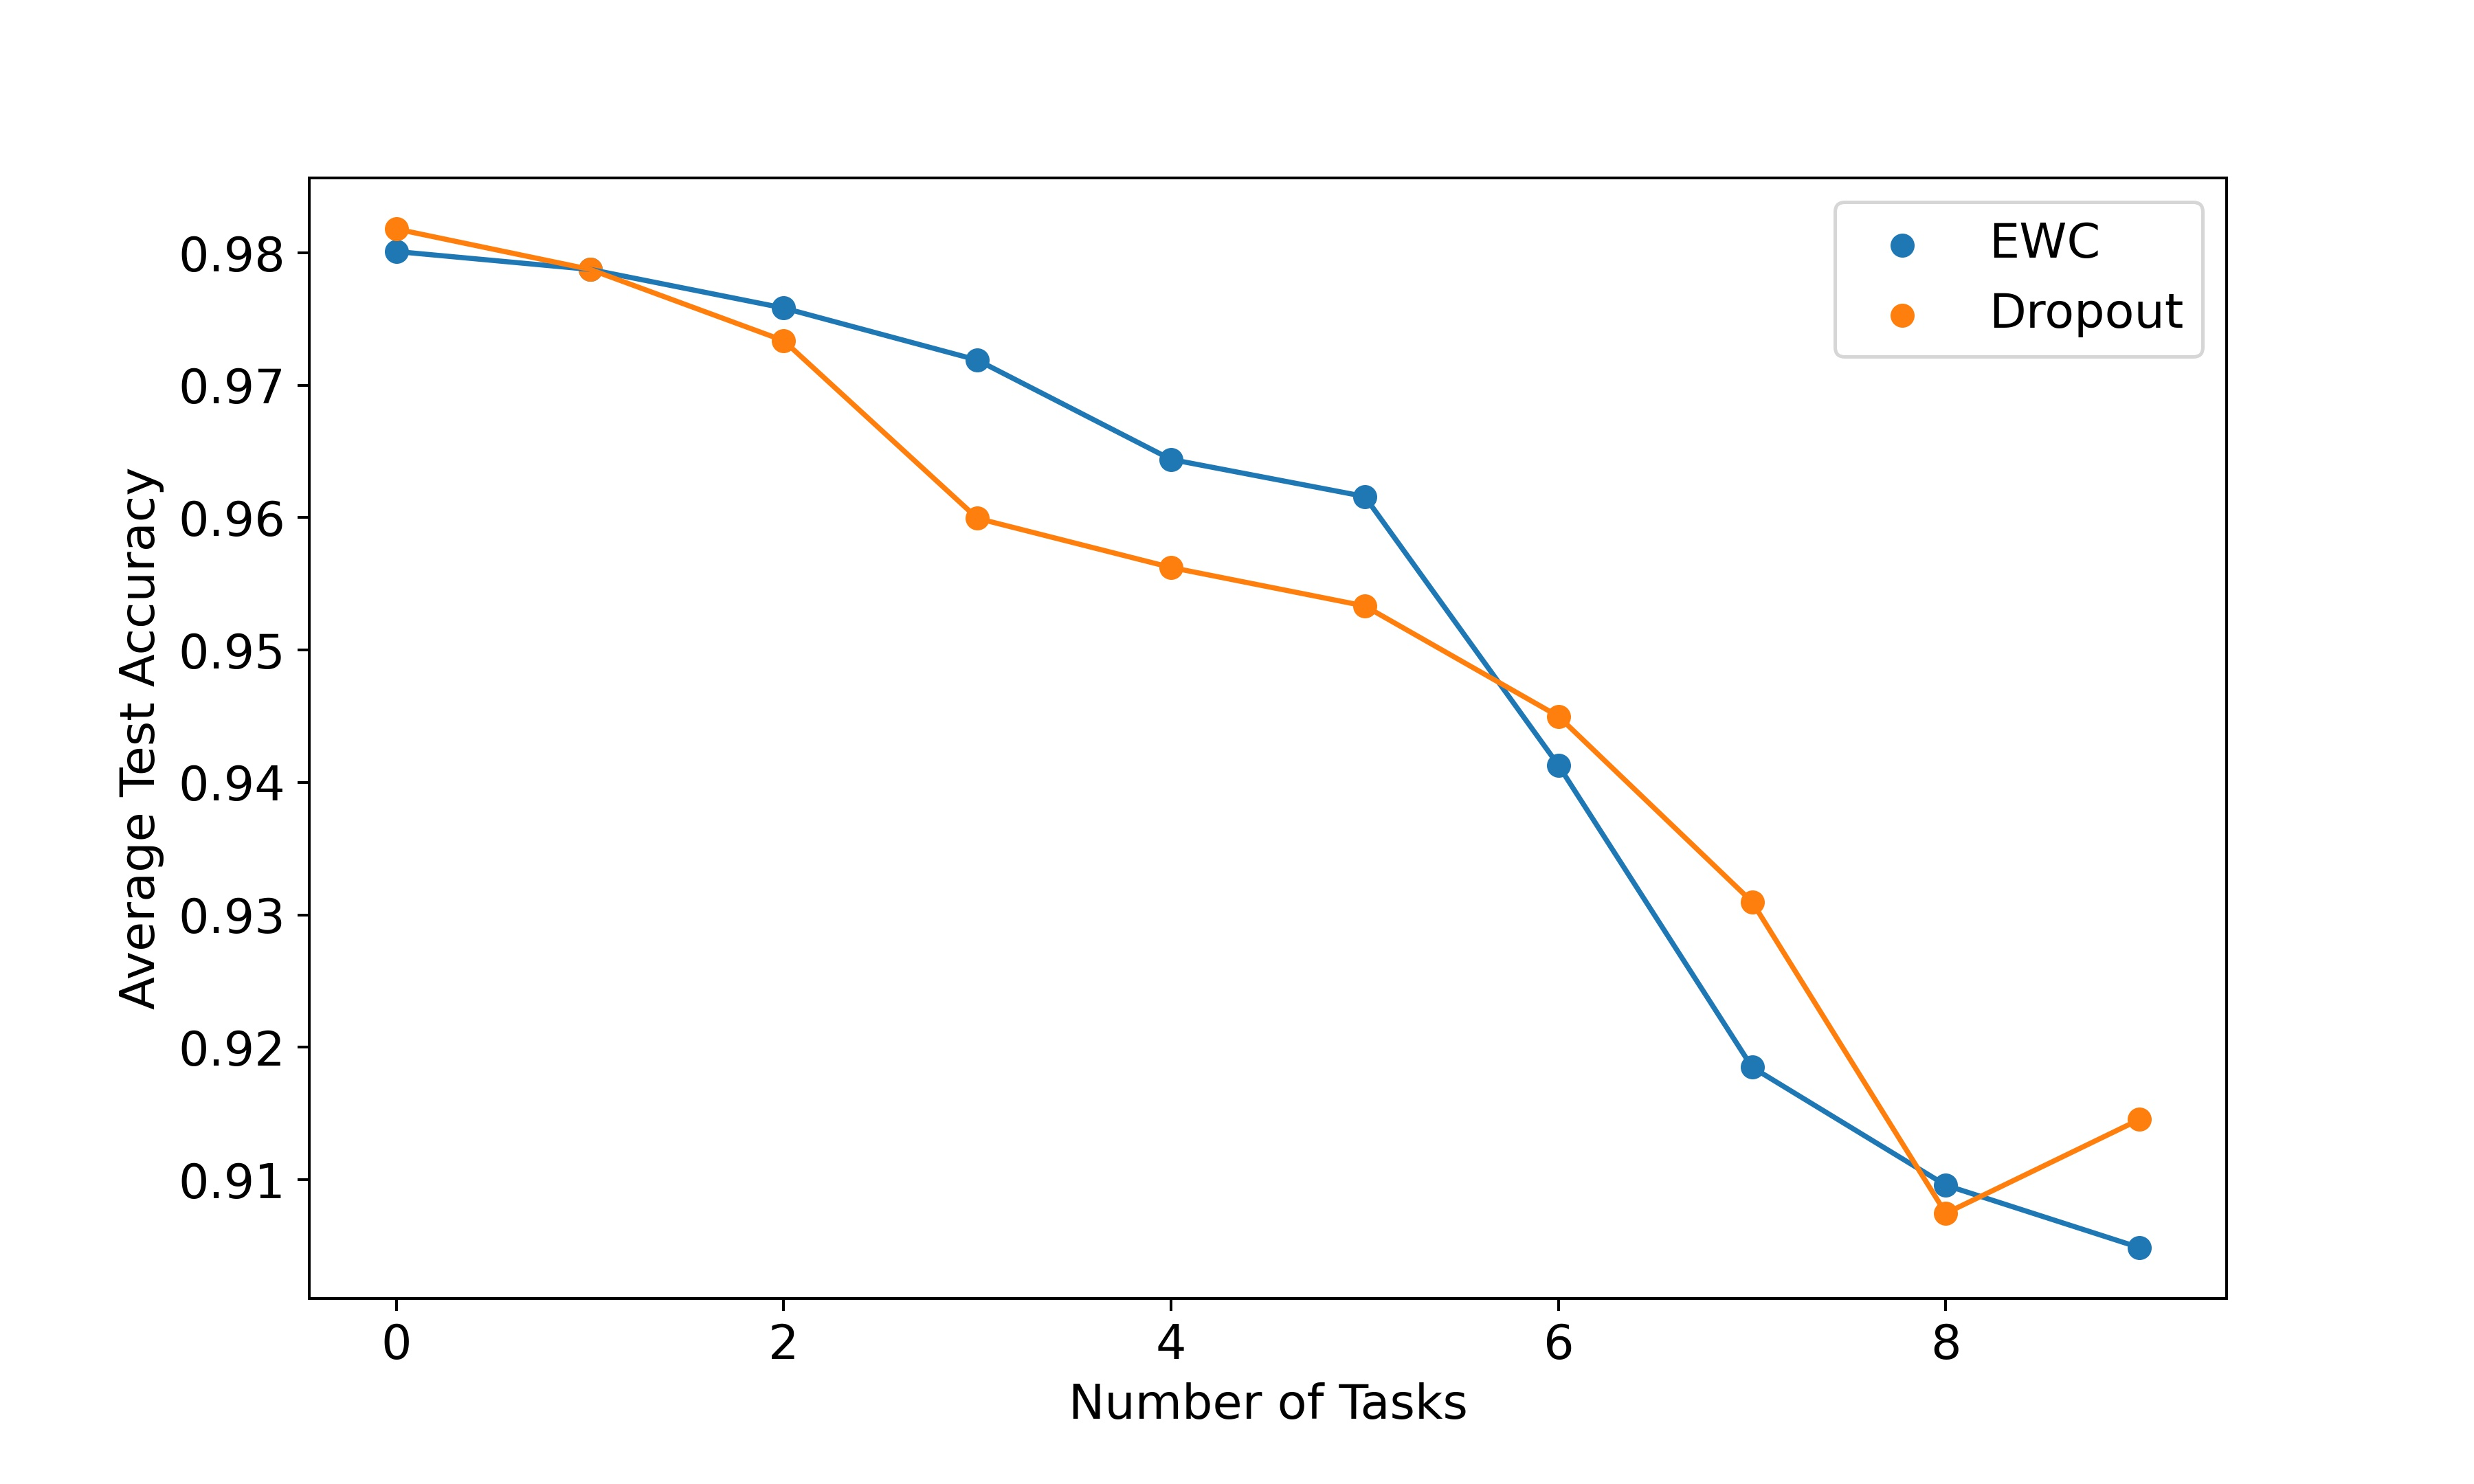
\includegraphics[width=\textwidth]{../Figures/Plot_b1.jpg}
         \caption{}
         \label{fig:repb}
     \end{subfigure}
     \hfill
     \begin{subfigure}[b]{0.32\textwidth}
         \centering
         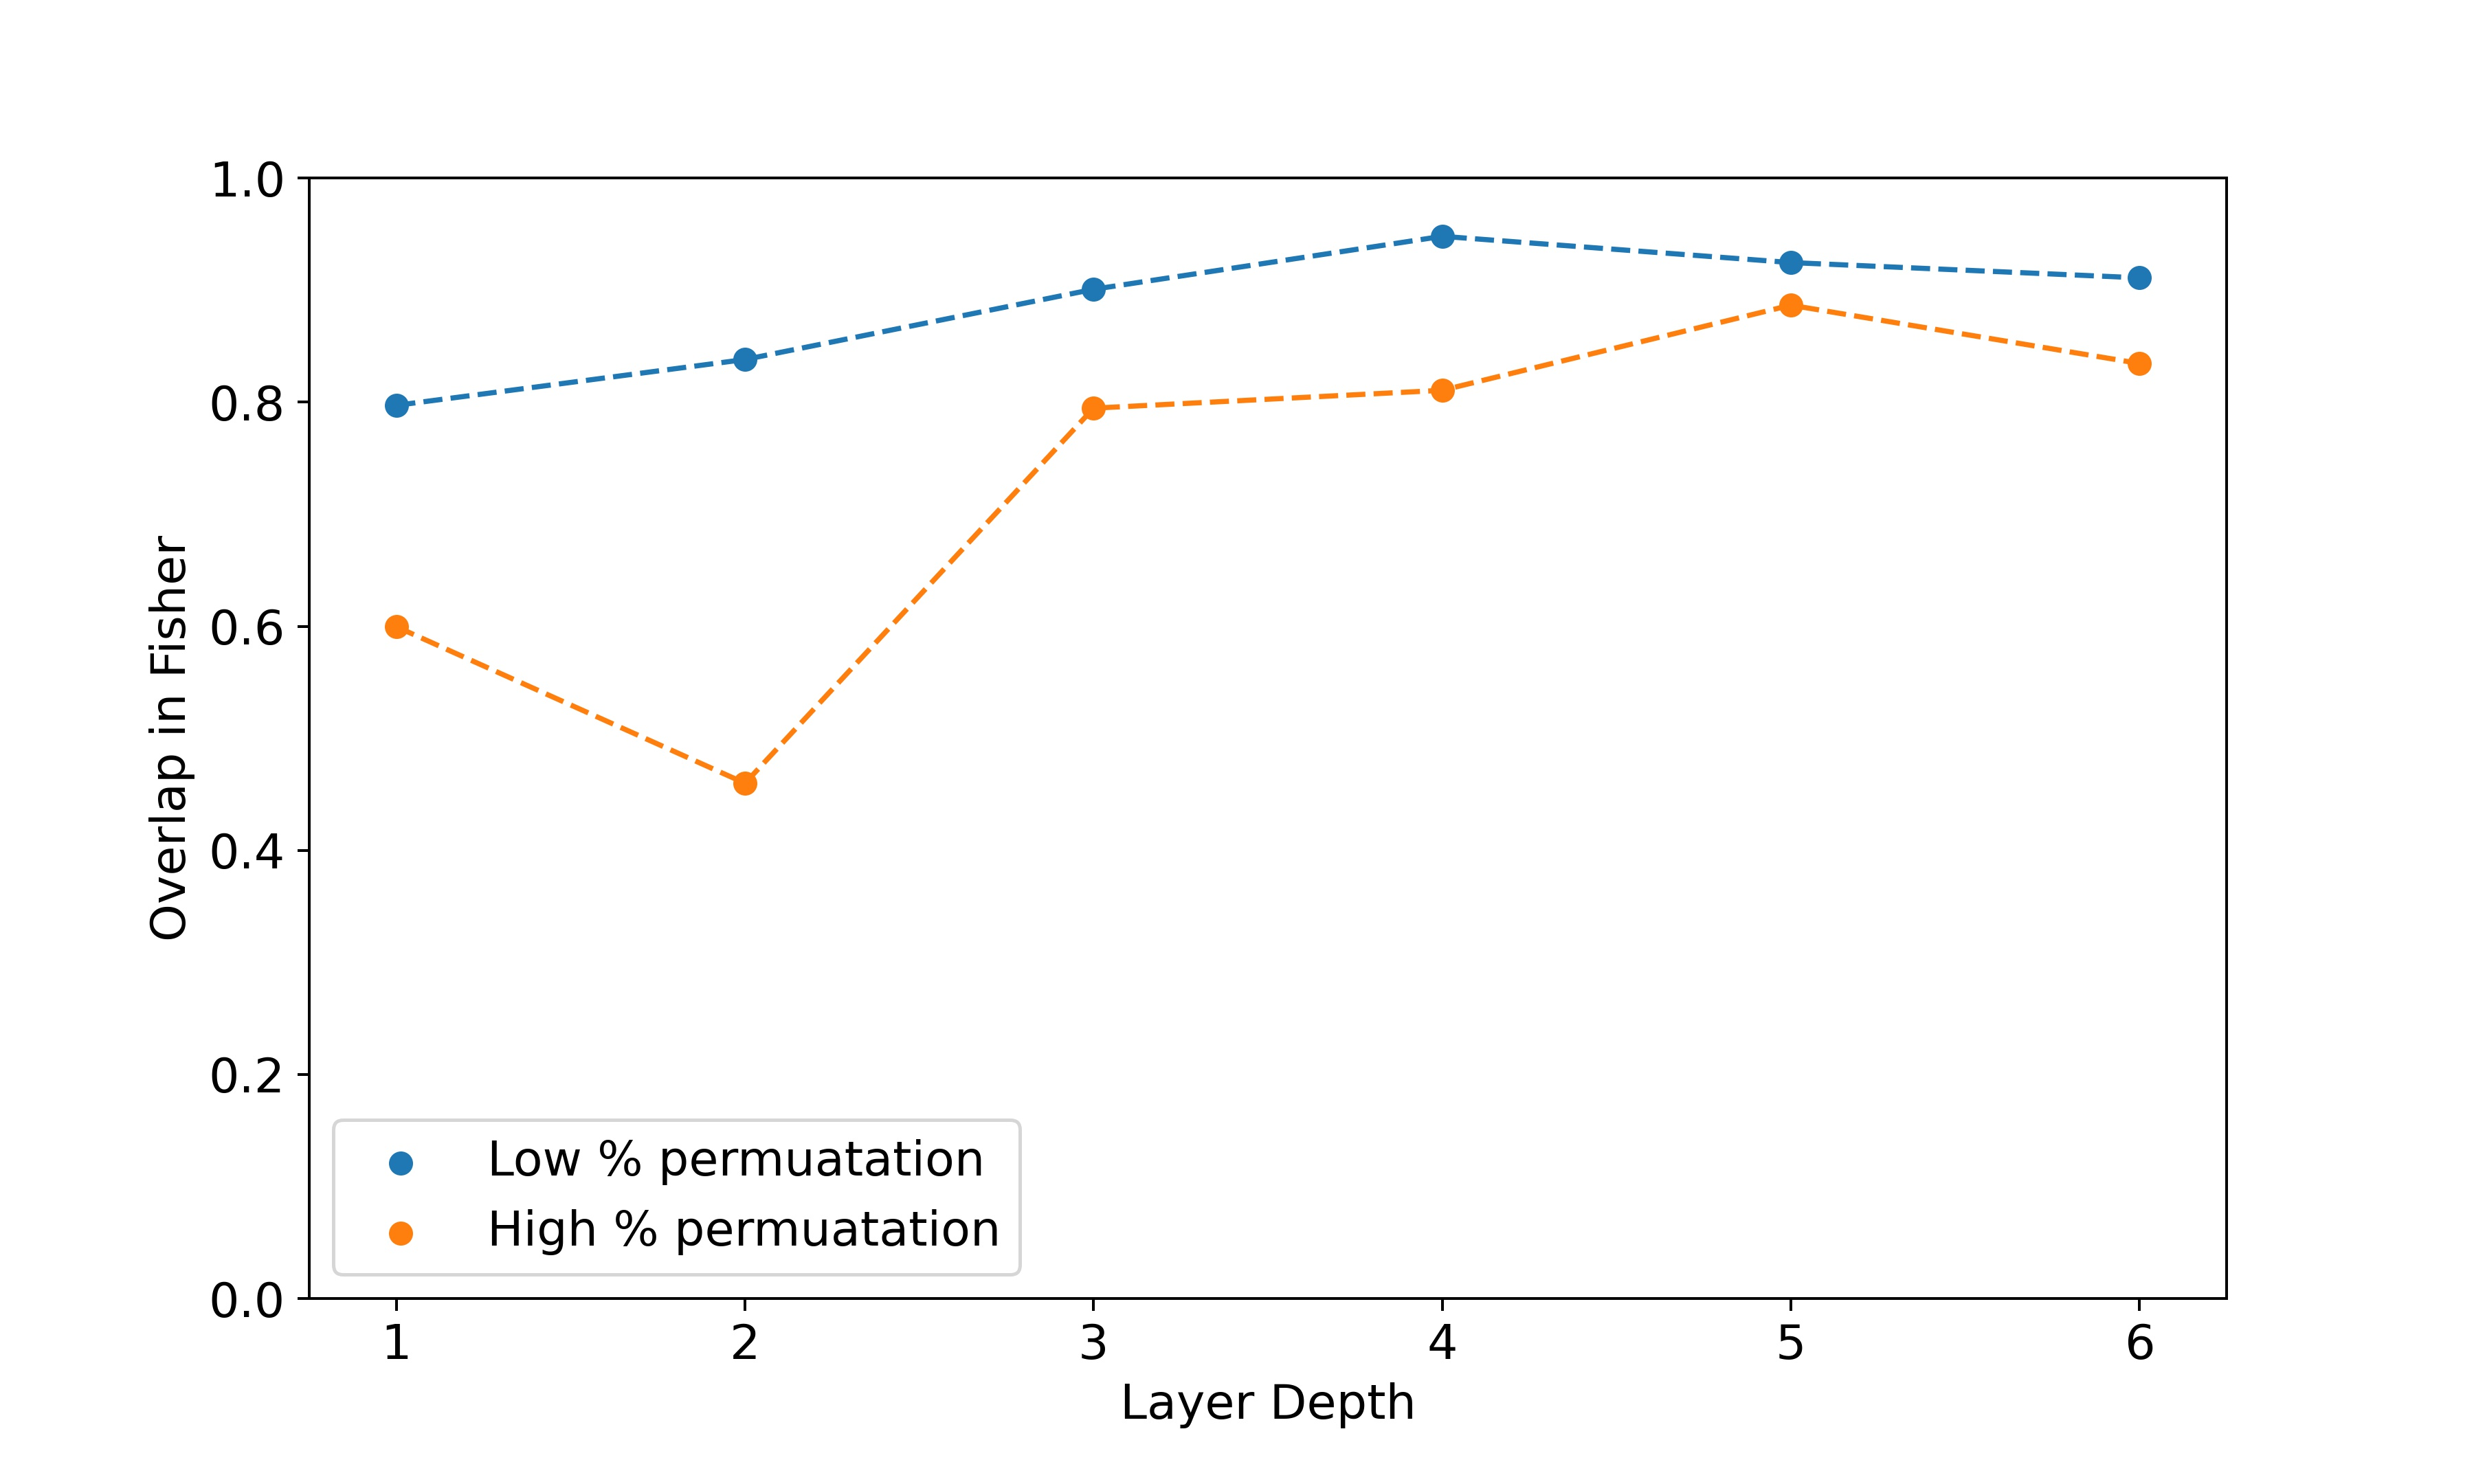
\includegraphics[width=\textwidth]{../Figures/Plot_c.jpg}
         \caption{}
         \label{fig:repc}
     \end{subfigure}
        \caption{Replication of the 3 MNIST Plots}
        \label{fig:rep}
\end{figure}

As can be seen in Figures \ref{fig:repa} and \ref{fig:repc}, both plots A and C could be replicated to a high level of accuracy. In Figure \ref{fig:repa}, we can see that EWC outperforms SGD on taskA once training on task B begins training, and the same could be said for tasks B and C. Further, L2 never achieves good performance on tasks B or C, the same as in the original paper. In addition, although the results in \ref{fig:repc} are not exactly the same as the original paper, the high permutation task has lower overlap in earlier layers, then catches up in the later layers. The overlap is also generally higher in later layers than earlier layers.

However, as we can see in \ref{fig:repb}, EWC seems to achieve siilar performance to Dropout after task 6. This is both because Dropout performs better than the results listed in the paper, and because EWC performs worse. It was hypothesized that the $\lambda$ value picked for EWC was too high, forcing the model to overprioritize earlier tasks. To remedy this, the same experiment was tried with $\lambda=0.005$.

\begin{figure}[!h]
\centering
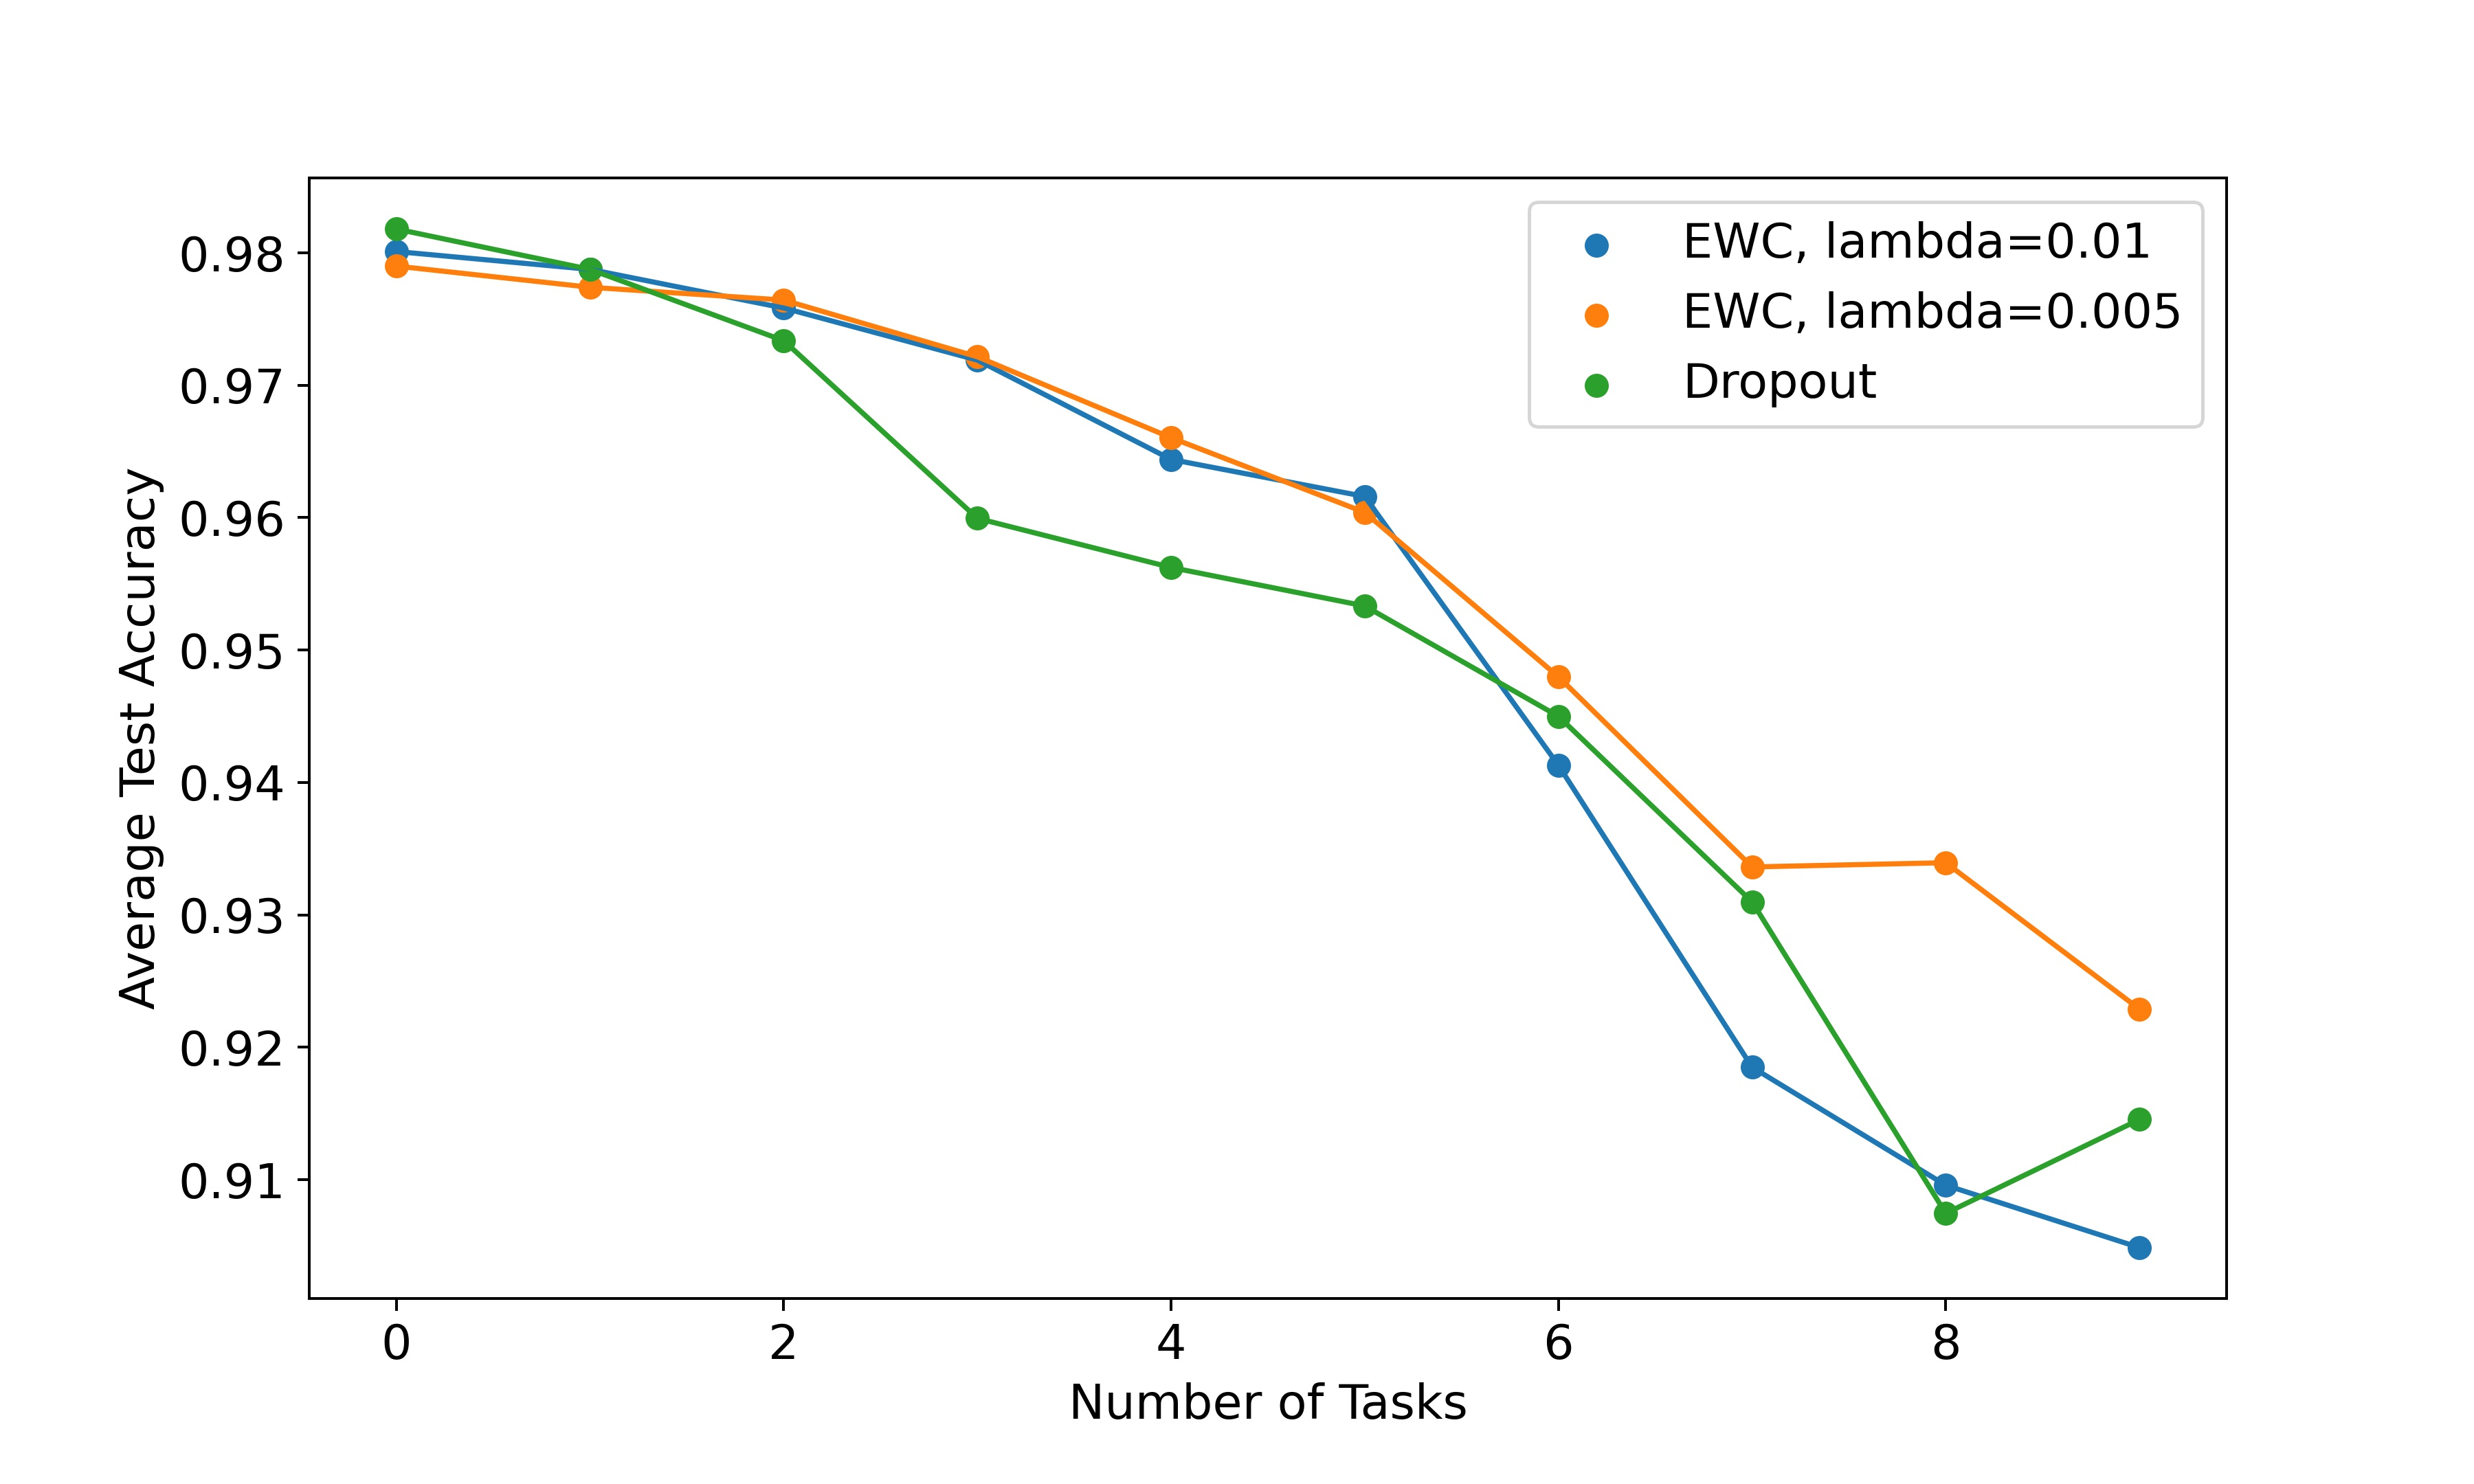
\includegraphics[width=0.5\textwidth]{../Figures/Plot_b2.jpg}
\caption{Plot B with both $\lambda=0.01$ and $\lambda=0.005$}
\label{fig:repb2}
\end{figure}

As can be seen in Figure \ref{fig:repb2}, using the lower value for $\lambda$ did allow EWC to achieve better performance than Dropout, but only to a small degree. Though this does not fully replicate the plot referenced in the original text, it does display the importance of tuning $\lambda$. Here we can see that tuning this hyperparameter can greatley impact performance. 




\bibliographystyle{unsrt}
\bibliography{neurips_2019}


\end{document}
